\chapter{\IfLanguageName{dutch}{Stand van zaken}{Quantum Essentials}}
\label{ch:quantum-essentials}

To make sure everyone starts off on the same baseline to understand the full potential of this paper, we will introduce a few of the basic quantum principles. This paper is not targeting these specific principles but does use them to explain different practical consequences of the use of them within quantum computation. If there is any further interest regarding these ground fundamentals, we would refer you to the following papers, ~\textcite{Rieffel1998} and ~\textcite{Shor2000}.

\subsection{The Qubit and its representations}

The foundation of any quantum related paper is and will always be the \textbf{qubit}. A qubit is just like a classical computing \textbf{bit} the foundational unit of its computer. Whilst a bit can either be on or off, a qubit has a certain statistical measurement to it. To be able to program on a quantum computer you need to think of the issue of computing an equation in a completely different way.

A qubit is not an infinite on or off, meaning that any type of computation needs to happen during the time frame qubit remaining stable without being thrown of its state by decoherence or any other external factors. 
One of the biggest issues with qubits is that they can behave unstable when influenced by the slightest of external influences, which also means the influence of an external observer. Once a qubit reaches an unstable state it has lost its quantum advantages and becomes a determined particle, which is not available for calculations any more. Meaning that during the execution of your program you are simply not able to look at the intermediary results as this would affect the final result, which would make the whole computation worthless. This means that debugging and looking at variables whilst you are executing a piece of code simply is not possible, which in turn makes writing actual code for a quantum computer a lot more difficult. This aspect will be explained more clearly further on.

First of all to comprehend the nature of a qubit we need to understand that representing a qubit is only possible in a complex field, which shows of a certain amplitude of the state of the qubit in a point in time. When we think about a classical bit, we like to imagine a switch being turned on or off. With a qubit you would have to think about a sphere that is being transformed and shifted around its axes to transform its state. \textit{Felix Bloch} was the individual that came up with the Bloch sphere that we currently use to clearly represent what a qubit is at a certain point in time. Looking at figure 2.1 you are able to see a representation of the state of a qubit in its elevated state. You need to think about this representation in a complex field on which transformations and rotations can be applied.
During runtime a qubit is in a probabilistic state where it can not be fully determined in which state the qubit currently resides, which makes the whole execution harder. The moment we measure the state of the qubit it will degrade back to a determined result that shows us exactly the state of the qubit.

\begin{figure}[h]
	\centering
	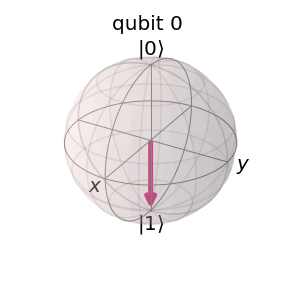
\includegraphics[scale = 0.75]{../Demonstration/img/Quantum_essentials_1.PNG}
	\caption{A Bloch sphere representation of a qubit in the $\ket{1}$ state. 
		The Bloch sphere clearly indicates that the state of a qubit has a certain complex aspect to it.}
\end{figure}

Another way of demystifying what a qubit exactly means is by representing it through the use of matrices and the Bra-ket notation. By using these matrices and using matrix transformations we can more easily expose the way a qubit can be influenced during execution. 
If you take a look at the way of representing a qubit in its elevated $\ket{1}$ state or base $\ket{0}$ state, by representing the qubits as a matrix we are able to more clearly show how operations on a quantum device have an impact on the state of the qubit.


\[
	\ket{0}=
	\begin{bmatrix}
	1					\\
	0
	\end{bmatrix} 
	and
	\ket{1}=
	\begin{bmatrix}
	0					\\
	1
	\end{bmatrix} 
\]
This image is mostly preferred by computer scientist because it gives them a clear image of transformation in the same way an ordinary logic gate can influence an electrical signal. The combination of qubit basis states can be achieved by the utilisation of a tensor product. In the formulae below you are able to see how a 2-qubit system is represented through their matrix-representation. So look at the following transformations in much the same way one would look at an electrical signal would flow through a set of gates. All transformations are applied by performing a Kronecker product on the 2 states. 

\[
\ket{00}=
\begin{bmatrix}
1					\\
0
\end{bmatrix} 
\otimes
\begin{bmatrix}
1					\\
0
\end{bmatrix} =
\begin{bmatrix}
1					\\
0					\\
0					\\
0					\\
\end{bmatrix}
\quad
\ket{01}=
\begin{bmatrix}
1					\\
0
\end{bmatrix} 
\otimes
\begin{bmatrix}
0					\\
1
\end{bmatrix} =
\begin{bmatrix}
0					\\
1					\\
0					\\
0					\\
\end{bmatrix}
\]
\[
\ket{10}=
\begin{bmatrix}
0					\\
1
\end{bmatrix} 
\otimes
\begin{bmatrix}
1					\\
0
\end{bmatrix} =
\begin{bmatrix}
0					\\
0					\\
1					\\
0					\\
\end{bmatrix}
\quad
\ket{11}=
\begin{bmatrix}
0					\\
1
\end{bmatrix} 
\otimes
\begin{bmatrix}
0					\\
1
\end{bmatrix} =
\begin{bmatrix}
0					\\
0					\\
0					\\
1					\\
\end{bmatrix}
\]

To sum it up a bit can be only be in a state of on or off and this can be checked throughout execution, whilst a qubit is in a uncertain state during execution much like Schrödinger's cat. So once we observe the qubit it becomes just as determined as a normal bit would be. But determining the state during execution will affect the rest of the experiment and will remove the potential benefits of quantum in much the same way if Schrödinger went on with the experiment after observation that the cat died, he would be certain that cat would still be dead at a later point.

\subsection{Superposition and entanglement}

Now the next 2 principles are fully responsible of giving quantum computing its exponential speed-up compared to classical computing in certain tasks like factorisation and database searches. However these principles only offer that powerful advantage when they operate together in solving a certain quantum algorithm. 

\textbf{Superposition} is a term a lot of people have heard about and how it could achieve major breakthroughs in the scientific world, but what it exactly represents is the real question.

We should think about qubits in superposition in a statistical way to receive a clearer picture. When a qubit is put into a state of superposition, the qubit operates between its elevated state and its ground state. By referring back to the representation of the Bloch sphere the qubit lives in a three dimensional complex field, where the only knowledge we can keep track of is its statistical chance of the state of the qubit. Until we have truly observed the qubit and have measured it extensively, the state of a qubit remains a statistical probability.

This all meaning that quantum particle can remain in both states at once whilst it has not been observed. To explain this more clearly from a computer science perspective, a qubit in superposition is during execution behaving as 0 and 1 at the same time. A concept that seems impossible within a classical frame of mind but also very advantageous if you know where to look. E.g. if you are processing a big array of data through your classical processor, your processor will take one item of the array, process, convert and output it before it will take another item of the array and perform the same thing. A quantum processor could go about this process in a similar yet much more ingenious way. It would put an amount of qubits in superposition to represent the full array as input, perform the needed amount of quantum gates and receive the output in a single go instead of needing to loop over the full array. ~\autocite{Draper2000}

\textbf{Entanglement} is another interesting principle within the realm of quantum physics. This principle truly offers the quantum advantage that is predicted over every single sector. 
It refers to the correlation between entangled qubits where the state of one qubit influences the state of the correlated qubit in a way that it can be exploited and theoretically infinitely speed up computation. This entanglement can be achieved inside a quantum computer by the use of quantum gates on qubits in a state of superposition. You are able to put every single qubit available in a entangled state with the qubits available in the system. By having this exponential factor inside your quantum system, it becomes more clear where the quantum advantage can truly be gained. Such a quantum system can represent an immense amount of classical bits by using this phenomenon. The deterministic result of the qubits at the end of an experiment will always show the correlation in the results, keeping in mind that enough experiments are performed to defend against quantum decoherence mistakes and other external influences.
~\autocite{fern2016mathematics}

These two principles are constantly being used  by a quantum processor as the one that Google showed of in their latest showcase of their quantum supremacy, ~\textcite{Google2019}. Together they are able to exponentially increase the computing power of a quantum computer, as you add more and more qubits you are exponentially increases the available data items such a processor could handle. For example to be able to simulate the biggest medicine of the 20th century, penicillin you would need 286 functional qubits, which in turn would be able to generate the $2^{286}$ bits of memory. It would straight up be impossible to get this amount of classical RAM, so it is impossible to simulate this medicine fully. Actually getting to such a stable amount of qubits in itself will still be a scientific miracle. The whole limitation of 'just adding qubits' to the system runs into a barrier by Quantum decoherence.

\subsection{Quantum decoherence}

QC is not solely composed of benefits, the biggest downside is that as of now technology has not yet progressed far enough to actually provide the necessary amount of stable qubits to perform trustworthy calculations with. For example the simulations of penicillin, a system would need 286 qubits that remain stable for a prolonged period, but as of now  Google has only been able to keep 53 qubits stable for a prolonged period of time using quantum error correction throughout the calculations. The loss of these quantum aspects during execution is called \textit{quantum decoherence}, it is the phenomenon that describes how a qubit falls in an unstable state after being influenced by external forces or even internal influences from the qubits around it inside the system.

Referring to figures 2.2 and 2.3 below you are able to see that quantum decoherence is even a measurable phenomenon. The circuit below is specially build to show that quantum decoherence even shows up in the smallest of computations, where a qubit gets thrown in an elevated state of $\ket{1}$ and then gets measured and pictured on a classical bit. If you analyse the results you are able to see that quantum decoherence has occurred and de-elevated the state of the qubit back to $\ket{0}$. In this specific case from the 1024 shots taking on the real quantum device, around 8 percent or 81 of the shots, were worthless due to the quantum decoherence.  

Taking all of this into account the whole field has one giant, non-circumventable downside that goes with it, the larger our quantum systems become, the more internal decoherence we receive from the higher concentration of qubits near each other. This all could mean that there is a limit to how big we are able to make quantum machines, because at a certain point, without proper error correction, the internal decoherence would make every single calculation useless because of the high probability of faulty data throughout. However if we are able to find a solution to this internal decoherence, the amount of qubits inside a system could be limitless and our data processing with it could also be limitless. \autocite{Hartnett2019}

It is of utmost importance that we add qubits in a controlled manner where we are able to perform better and better error-correction before we just add more qubits in the system. If everyone started adding qubits to their systems without performing any research regarding quantum error correction, we would only receive an increase in computing power with more unreliable results. And in this case quality is a way more important factor compared to brute quantity. 

\begin{figure}[h]
	\centering
	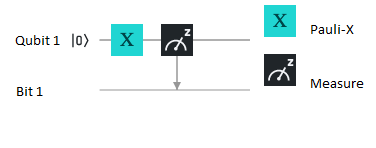
\includegraphics[scale = 0.75]{../Demonstration/img/Quantum_decoherence_circuit.PNG}
	\caption{This is the quantum circuit that puts a qubit in an elevated state followed up with a measurement, to show off how quantum decoherence can influence the results.}
\end{figure}

\begin{figure}[h]
	\centering
	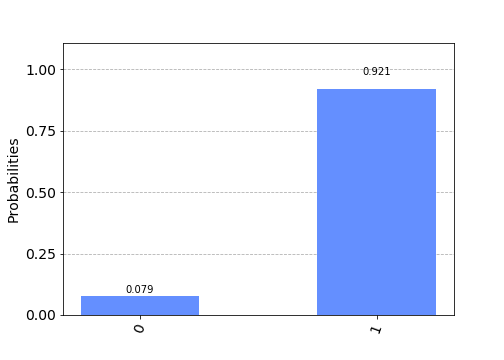
\includegraphics[scale = 0.75]{../Demonstration/img/Quantum_decoherence_graph.PNG}
	\caption{These are the results from which it is clearly visible that quantum decoherence has taken place on the initial $\ket{1}$ state to the $\ket{0}$ state.}
\end{figure}



\subsection{Quantum gates}

Now one might wonder, how do we create calculations with particles that are not observable and not tangible at a point in time. Quantum gates offer the solution to this question, a quantum gate affects one or more qubits during execution so that a programmer is able to perform changes to the state of the qubit but does not create an unstable qubit. From a programmers perspective they function in a similar way that a normal logic gate functions on an electrical signal inside a regular processor. Furthermore we will provide some frequently used quantum gates. One major difference rule that a quantum computer has to listen to when it comes to its gates, is that quantum have to be 100 percent reversible while a classical computer does not have to deal with this limitation. This is clearly shown by the use of matrix representations when a qubit passes through a specific quantum gate and for a classical example, thing of an OR-gate you are able to see the outcome of the signal with an on or an off, but you can not know just from the outcome which initial signal influenced the OR-gate to be activated.

To understand the application of quantum gates inside a circuit on qubits, we would like to refer back to the representation of matrices where transformations are applied by performing a Kronecker product on the qubit in question.

\subsubsection{Hadamard gate}
The Hadamard gate is single most important gate for creating a quantum computation. This gate is responsible for putting a qubit inside a state of superposition and is also the one to get it out of this state. So in turn without this gate, quantum advantage would not exist. It maps  $\ket{0}$ to $\frac{\ket{0} + \ket{1}}{\sqrt{2}}$ and $\ket{1}$ to $\frac{\ket{0}-\ket{1}}{\sqrt{2}}$, which are both superposition states.

\[
H=\frac{1}{\sqrt{2}}\begin{bmatrix}
1 & 1 \\
1 & -1
\end{bmatrix}
\]

\subsubsection{Pauli-X gate}
Performs in a similar way a classical NOT-gate performs on an electrical signal or an absence of it. A qubit in $\ket{0}$ state going through a Paul-X gate would go in a $\ket{1}$ state.

\[
X=
\begin{bmatrix}
0 & 1 \\
1 & 0
\end{bmatrix}
\]

\subsubsection{CNOT gate}
This gate works as a flip for a qubit. It is connected to 1 control qubit marked with an X and targets a target qubit marked with a small circle. If the control qubit is in an activated state it will flip the target qubit.

 \[
 CNOT=
 \begin{bmatrix}
 1 & 0 & 0 & 0 \\
 0 & 1 & 0 & 0 \\
 0 & 0 & 0 & 1 \\
 0 & 0 & 1 & 0 \\	
 \end{bmatrix}
 \]

\subsubsection{Toffoli, CCNOT gate}
The Toffoli gate works in the same way as a CNOT gate, but instead it has 2 control qubits. So both of them need to be activated to actually flip the target qubit, which logically requires at least 3 qubits in your system. This gate is the connector of the whole quantum system where we are able to entangle superposition states.

 \[
CCNOT=
\begin{bmatrix}
1 & 0 & 0 & 0 & 0 & 0 & 0 & 0\\
0 & 1 & 0 & 0 & 0 & 0 & 0 & 0\\
0 & 0 & 1 & 0 & 0 & 0 & 0 &  0\\
0 & 0 & 0 & 1 & 0 & 0 & 0  & 0\\
0 & 0 & 0 & 0 & 1 & 0 & 0  & 0\\
0 & 0 & 0 & 0 & 0 & 1 & 0  & 0\\
0 & 0 & 0 & 0 & 0 & 0 & 0 & 1 \\
0 & 0 & 0 & 0 & 0 & 0 & 1 & 0\\
\end{bmatrix}
\]

This is just a listing of the most prevalent quantum gates. These quantum gates form the bases for performing the simplest of quantum algorithms, which can be implemented through a programming interface or through many of the UI-editors where you can add gates along the circuit in a dynamic way. You are even able to send off these generated circuits through the UI tools off to real devices or simulators to analyse and compare your results.



